\documentclass[journal]{IEEEtran}
\usepackage{amsmath}
\usepackage{booktabs}
\usepackage{graphicx}
\usepackage{cite}
\usepackage{hyperref}
\usepackage{array}
\usepackage{multirow}
\usepackage{tabularx}

\newcolumntype{L}{>{\raggedright\arraybackslash}X}
\graphicspath{ {./images/} }
\begin{document}

\title{Proactive TCP Congestion Control Using Machine Learning-Driven Artificial ECN Signals}

\author{Bhuvanakshi~LN,
        Brijesh~Shetty~N,
        Chinami~Datta~Ram,
        Hemanth~Kumar~K,
        and~Nalina~V%
\thanks{All authors are with the Department of Information Science and Engineering,
B.M.S. College of Engineering, Bengaluru, India.
Emails: bhuvanakshi.is23@bmsce.ac.in, brijesh.is23@bmsce.ac.in,
chinami.is23@bmsce.ac.in, hemanth.is23@bmsce.ac.in, nal.ise@bmsce.ac.in}}

\maketitle

\begin{abstract}
Traditional TCP congestion control algorithms such as Reno and Cubic react to packet loss only after it has occurred, resulting in performance degradation through retransmissions and reduced throughput. This paper presents a proactive artificial Explicit Congestion Notification (ECN) framework that uses LightGBM to detect the onset of TCP congestion in real time and responds with proportional adjustments to RED queue thresholds scaled to prediction confidence. A dataset of 57,808 samples is extracted from 300 Mininet experiments spanning a $5\times5\times3\times2$ network parameter grid (bandwidth, delay, BDP, CC algorithm), and labeled using a multi-signal consensus strategy---simultaneously requiring CWND drop, ssthresh engagement, and retransmission activity---to produce a naturally balanced dataset free of data leakage. A single LightGBM model trained on the combined Reno and Cubic dataset identifies the congestion state with F1\,=\,0.9723 and ROC-AUC\,=\,0.9965; cross-evaluation (training on one CC variant and testing on the other) confirms that the unified model generalizes across Reno and Cubic (F1\,$\approx$\,0.94), and a forward-looking variant anticipates loss within the next $\sim$40\,ms. Mininet deployment experiments show that the proportional ECN mechanism eliminates 100\% of retransmissions for TCP Cubic ($755\!\rightarrow\!0$) and achieves a 15.5\% throughput improvement for TCP Reno.
\end{abstract}

\begin{IEEEkeywords}
TCP congestion control, LightGBM, Explicit Congestion Notification (ECN), packet loss prediction, RED queue management, Mininet, proactive congestion control
\end{IEEEkeywords}

% -------------------------------------------------------------------
\section{Introduction}
% -------------------------------------------------------------------

Traditional TCP congestion control algorithms---most notably Reno~\cite{rfc5681} and Cubic~\cite{rfc9438}---operate on a strictly loss-based feedback loop. The sender increases its congestion window (\emph{cwnd}) until packets are dropped, uses that drop as the congestion signal, and then halves (Reno, $\beta=0.5$) or scales back (Cubic, $\beta=0.7$) its rate. This reactive paradigm inherently requires network queues to overflow before corrective action is taken, generating retransmissions that degrade throughput, inflate round-trip time (RTT), and reduce Quality of Experience (QoE) for end users.

Explicit Congestion Notification (ECN)~\cite{rfc3168} offers a pathway for routers to signal impending congestion before queues overflow, enabling TCP to back off gracefully. However, ECN effectiveness depends on the accuracy and timeliness of the congestion signal. Active Queue Management (AQM) schemes such as RED mark packets probabilistically based on average queue length---a coarse, threshold-based heuristic that cannot anticipate congestion at the granularity of individual TCP flows and round-trip times.

Machine learning (ML) offers the ability to extract fine-grained predictive congestion signals from TCP state variables---congestion window size, RTT, slow-start threshold, retransmission counters, and their temporal derivatives---that are directly observable at the sender. If a model can reliably predict an imminent loss event several RTTs ahead, a proactive ECN signal can trigger a graceful \emph{cwnd} reduction and avoid the packet drop entirely. Recent work by Welzl et al.~\cite{welzl2024} demonstrated the feasibility of real-time TCP loss prediction using gradient-boosted trees on Mininet-emulated flows, establishing an important proof-of-concept for this direction.

Building on this foundation, this paper makes the following contributions:
\begin{itemize}
  \item A leak-free multi-signal consensus labeling strategy requiring simultaneous CWND drop ($\geq30\%$), ssthresh engagement, and retransmission activity, producing a naturally balanced dataset (48.07\% loss / 51.93\% normal) across 300 Mininet experiments spanning delays of 30--70\,ms and bandwidths of 10--50\,Mbit/s.

  \item A single LightGBM model trained on the combined Reno\,+\,Cubic dataset with \textbf{71 candidate features} (rolling statistics, temporal differentials, lags, ratios, and interaction terms), reduced to \textbf{45 features} after automated selection, with 7-fold TimeSeriesSplit validation and Optuna hyperparameter tuning---detecting the congestion state at F1\,=\,0.9723 and generalizing across both CC variants (cross-CC F1\,$\approx$\,0.94) without separate per-algorithm models.

  \item A proportional RED threshold adjustment mechanism (\texttt{tc qdisc change}) that scales the congestion response to LightGBM prediction confidence, enabling graduated queue management rather than binary ECN toggling.

  \item Mininet validation demonstrating 100\% retransmission elimination for TCP Cubic and $+15.5\%$ throughput for TCP Reno, with the proportional model outperforming both baseline TCP and binary ECN approaches.
\end{itemize}

The remainder of this paper is organized as follows. Section~\ref{sec:related} reviews related work. Section~\ref{sec:method} describes the proposed system. Section~\ref{sec:results} presents experimental results and discussion. Section~\ref{sec:conclusion} concludes.

% -------------------------------------------------------------------
\section{Literature Review}
\label{sec:related}
% -------------------------------------------------------------------

The intersection of machine learning and TCP congestion control has been explored across a spectrum of problem formulations, ranging from coarse network-wide congestion forecasting to fine-grained per-flow loss prediction at transport-layer timescales.

Early ML-based congestion detection work focused on network-level classification. Decision Tree, Random Forest, and ANN models applied to OPNET simulation data in mobile ad-hoc networks (MANETs) achieved prediction precision of 98.7--99.8\%, though on synthetic data without empirical mitigation validation~\cite{manet}. Similarly, XGBoost classifiers with SMOTE-based class balancing on real ISP warehouse data (23,000\,+ interfaces) demonstrated 30-day congestion prediction windows at 0.976--0.986 accuracy, but without any closed-loop control response~\cite{ptcl}. For enterprise networks, Spatiotemporal Graph Convolutional Networks (ST-GCN) on ESnet telemetry achieved F1\,=\,0.916 with 20-minute prediction horizons, though scalability beyond 10,000 nodes remains unaddressed~\cite{stgcn}.

Classification approaches for packet loss type identification have distinguished congestive from non-congestive losses in hybrid wired-wireless topologies using Random Forest, KNN, and Gradient Boosting in ns-3 simulations, achieving F1 scores of 0.88--0.89~\cite{ali2024}. While these methods identify the type of loss accurately, they operate reactively---triggering only after loss has already occurred. Traffic volume forecasting using ARIMA, MLP, and LSTM models integrated with SDN controllers~\cite{labonne} and GRU-based deep learning on the WIDE real-world dataset (MAPE\,$\approx$\,6.57\%)~\cite{wide2025} enable proactive resource allocation, but predict aggregate traffic volume rather than binary per-flow loss events, operating at timescales of minutes rather than per-RTT milliseconds.

Reinforcement learning (RL) has been extensively applied to dynamic congestion window control. RL-based TCP mechanisms integrated with ns-3 and OpenAI Gym demonstrated 81\% throughput improvement in wireless mesh networks~\cite{rl_mesh}, and Deep Q-Network (DQN) approaches achieved 46.29\% RTT reduction versus TCP Cubic in heterogeneous environments~\cite{dqn_tcp}. However, RL-based schemes adjust \emph{cwnd} reactively in response to observed network state rather than predicting future loss, and their computational overhead poses barriers to end-host deployment. Intelligent AQM systems combining LSTM prediction with Q-learning-based dynamic tuning on CAIDA traces improved throughput/RTT ratios and reduced buffer occupancy~\cite{aqm_lstm}, while XGBoost with Remora Optimization on NS2 features reached 96\% accuracy at the transport layer~\cite{remora}---yet neither couples predictions to proportional ECN signaling.

The survey by Tafa and Milutinovic~\cite{tafa_survey} identifies a persistent gap: despite the breadth of ML approaches, the field lacks systems that close the loop between fine-grained real-time binary loss prediction and proportional congestion response at per-RTT timescales. Specialized applications in Content-Centric Networks~\cite{ccn} and Wireless Sensor Networks~\cite{wsn} confirm that predictive approaches can reduce queue overflow and improve QoS, but operate at coarser timescales and do not generalize to standard TCP environments.

The most directly related prior work is Welzl et al.~\cite{welzl2024}, who presented the first real-time TCP packet loss prediction system using XGBoost models trained on Mininet-emulated Reno and Cubic flows. Their system polls TCP state via \texttt{ss}, predicts binary loss, and injects ECN signals at the sender. Our work extends this concept with a leak-free labeling strategy, a unified model across CC variants, richer feature engineering, calibrated thresholds, and proportional RED threshold adjustment achieving F1\,=\,0.9723 and demonstrably superior real-network results.

% -------------------------------------------------------------------
\section{Proposed Method}
\label{sec:method}
% -------------------------------------------------------------------

This section describes the end-to-end system architecture: (A) network topology and data collection, (B) leak-free dataset construction and labeling, (C) feature engineering, (D) model training and selection, (E) the proportional artificial ECN mechanism, and (F) the complete system implementation flowchart.

\subsection{Network Topology and Data Collection}

We adopted a Mininet dumbbell topology with a single bottleneck link, following standard practice in TCP congestion research~\cite{welzl2024}. One foreground iPerf3 sender (h1) transmits to a receiver (h3) across two switches (s1--s2); six background flows compete for the same bottleneck to simulate realistic Internet competition. The bottleneck capacity is set to 10\,Mbit/s with HTB (Hierarchical Token Bucket) shaping. Netem delay of 15\,ms is applied on each host-facing interface, yielding a deployment RTT of 30\,ms. During training data collection, the delay parameter was varied from 30--70\,ms across the parameter grid.

TCP state data were collected using the Linux \texttt{ss -tin} utility, polled every 20\,ms at a fixed interval. Each sample captures: \emph{cwnd}, \emph{ssthresh}, RTT and RTT variance (\emph{rttvar}), retransmission counters, unacked segments, bytes sent, pacing rate, and timer information. We executed 300 experiments across a parameter grid of 5 bandwidths (10--50\,Mbit/s) $\times$ 5 delays (30--70\,ms) $\times$ 3 BDP multipliers (0.5$\times$, 1$\times$, 2$\times$) $\times$ 2 CC algorithms (Reno, Cubic), run at both 100\,s and 300\,s durations, yielding 150 Cubic and 150 Reno experiment folders. A fixed background traffic configuration was used to maximize temporal depth per parameter set.

\subsection{Dataset Construction and Leak-Free Labeling}

A critical challenge in TCP loss prediction is avoiding data leakage: if the training label is derived directly from a field (e.g., \texttt{lost\,>\,0}) that describes the outcome being predicted, the model effectively reads the answer rather than learning predictive behavior. Naive labeling based on the \texttt{lost} field produces only 14.93\% positive class (8,632\,/\,57,808 rows), creating severe class imbalance and a classifier that cannot generalize.

To address this, we designed a \emph{Multi-Signal Consensus Labeling} strategy. A sample is labeled as a congestion event (class 1) if and only if at least two of the following three signals are simultaneously active:
\begin{itemize}
  \item \textbf{Signal 1 --- CWND Drop:} the congestion window dropped $\geq30\%$ from its rolling 5-sample peak, indicating the TCP stack has reacted to congestion.
  \item \textbf{Signal 2 --- ssthresh Active:} \texttt{cwnd\,$\leq$\,ssthresh\,$\times$\,1.2} AND \texttt{ssthresh\,>\,0}, indicating the slow-start threshold is throttling window growth.
  \item \textbf{Signal 3 --- Retransmission:} \texttt{retrans\_now\,>\,0} OR \texttt{lost\,>\,0} OR \texttt{retrans\_diff\,>\,0}, indicating actual packet loss or retransmission activity at this instant.
\end{itemize}

Although Signal~3 references the \texttt{lost} column, labeling is performed entirely as a preprocessing step before any model training, after which all leakage-prone columns---\texttt{lost}, \texttt{retrans\_now}, \texttt{retrans\_total}, \texttt{retrans\_diff}, \texttt{bytes\_retrans}, and \texttt{sacked}---are removed from the feature set. The classifier therefore learns exclusively from TCP flow dynamics. This consensus approach naturally balances the dataset: 27,790 loss events (48.07\%) vs.\ 30,018 normal events (51.93\%) across 57,808 total samples, eliminating the need for aggressive oversampling.

\subsection{Feature Engineering}
\label{sec:features}

Raw \texttt{ss} output provides approximately 25 base TCP metrics per sample. From these, we engineered \textbf{71 candidate features} organized into five groups. After automated feature selection---variance threshold filtering and removal of features with pairwise Pearson correlation $>0.98$---\textbf{45 features} were retained for model training:

\textbf{Rolling statistics:} 5-sample rolling mean and standard deviation of \emph{cwnd}, RTT, \emph{ssthresh}, and unacked segments (e.g., \texttt{cwnd\_roll5\_mean}, \texttt{rtt\_roll3\_mean}), capturing recent metric trajectories rather than instantaneous values.

\textbf{Temporal differentials:} First-order differences (\texttt{cwnd\_diff}, \texttt{rtt\_diff}) and second-order accelerations (\texttt{cwnd\_accel}, \texttt{rtt\_accel}), encoding the rate and direction of change---critical for detecting the inflection point preceding a loss event.

\textbf{Lag features:} Previous 1- and 2-sample values of \emph{cwnd} and RTT (\texttt{cwnd\_lag1}, \texttt{cwnd\_lag2}, \texttt{rtt\_lag1}, \texttt{rtt\_lag2}), providing explicit short-term memory without requiring recurrent model architectures.

\textbf{Ratio features:} \texttt{retrans\_ratio}, \texttt{ack\_ratio}, \texttt{rtt\_ratio}, \texttt{cwnd\_util}---normalizing each metric relative to its recent range, making features scale-invariant across different network parameter configurations.

\textbf{Interaction features:} \texttt{cwnd\_rtt\_interaction} (product of \emph{cwnd} and RTT, proportional to bytes in flight), \texttt{buffer\_fill\_ratio} (estimated queue occupancy), and \texttt{congestion\_signal} (composite indicator), capturing non-linear co-variation that individual features cannot express.

This rich feature set adds temporal depth and relational context beyond raw \texttt{ss} output, substantively improving class separability---as confirmed by the resulting F1\,=\,0.9723 on the combined Reno\,+\,Cubic model. This performance is jointly attributable to the leak-free labeling strategy, comprehensive feature engineering, and class-balanced training.

\begin{table}[!t]
\renewcommand{\arraystretch}{1.3}
\caption{Final Dataset Statistics}
\label{tab:dataset}
\centering
\begin{tabular}{lr}
\toprule
\textbf{Metric} & \textbf{Value} \\
\midrule
Total rows & 57,808 \\
Features engineered                    & 71 \\
Features retained (after selection)    & 45 \\
Loss events (class 1) & 27,790 (48.07\%) \\
Normal events (class 0) & 30,018 (51.93\%) \\
Reno samples & $\sim$28,900 \\
Cubic samples & $\sim$28,900 \\
Experiments & 300 (150 Cubic + 150 Reno) \\
Parameter grid & 5 BW $\times$ 5 delay $\times$ 3 BDP $\times$ 2 CC \\
\bottomrule
\end{tabular}
\end{table}

\subsection{Model Training and Selection}

Six classifiers are reported here; eight were evaluated in total. KNN (F1\,=\,0.83), Decision Tree (F1\,=\,0.89), and Naive Bayes (F1\,=\,0.48) were excluded due to substantially lower F1-scores. The six highest-performing classifiers evaluated on the combined 57,808-row Reno\,+\,Cubic dataset are: Gradient Boosting, Random Forest, XGBoost, LightGBM, CatBoost, and a Stacking Ensemble (meta-learner: Logistic Regression). Training on the combined dataset tests whether a single model generalizes across both Reno and Cubic behavior. All models were trained under the following unified configuration:

\begin{itemize}
  \item \textbf{Validation:} 7-fold TimeSeriesSplit to preserve temporal ordering and prevent future-data leakage across folds.
  \item \textbf{Class balancing:} BorderlineSMOTE applied only on training folds (never on validation), oversampling near the decision boundary.
  \item \textbf{Hyperparameter tuning:} Optuna framework with 30 trials each for XGBoost and LightGBM, optimizing F1-score via 3-fold TimeSeriesSplit within each trial. Other models (GradientBoosting, RandomForest, CatBoost, StackingEnsemble) used manually configured hyperparameters.
  \item \textbf{Threshold calibration:} Per-fold F1-maximizing search on \texttt{predict\_proba} output, rather than the conventional fixed 0.5 default.
\end{itemize}

\begin{table}[!t]
\renewcommand{\arraystretch}{1.3}
\caption{Model Comparison --- Combined Dataset (57,808 Rows)}
\label{tab:models}
\centering
\begin{tabular}{lccccc}
\toprule
\textbf{Model} & \textbf{Acc.} & \textbf{F1} & \textbf{ROC-AUC} & \textbf{PR-AUC} & \textbf{Thr.} \\
\midrule
GradBoost      & 0.9473 & 0.9439 & 0.9895 & 0.9885 & 0.41 \\
RandomForest   & 0.9272 & 0.9230 & 0.9822 & 0.9810 & 0.45 \\
XGBoost        & 0.9690 & 0.9670 & 0.9957 & 0.9951 & 0.38 \\
LightGBM $\star$ & 0.9740 & 0.9723 & 0.9965 & 0.9960 & 0.38 \\
CatBoost       & 0.9694 & 0.9674 & 0.9953 & 0.9947 & 0.40 \\
StackEnsemble  & 0.9685 & 0.9664 & 0.9903 & 0.9889 & 0.45 \\
\bottomrule
\multicolumn{6}{l}{$\star$ Selected for deployment.}
\end{tabular}
\end{table}

LightGBM achieved the highest F1 (0.9723) and ROC-AUC (0.9965) and was selected for deployment. The per-fold training threshold of 0.38 was re-calibrated to 0.56 on the deployment network to balance sensitivity against false-positive ECN triggering. The balanced dataset (48\% positive) yields a naturally moderate threshold, reflecting a well-separated class distribution.

\subsection{Proportional Artificial ECN Mechanism}

Existing binary ECN approaches toggle congestion signaling fully on or off regardless of prediction confidence, offering no proportionality to the degree of predicted congestion. Our mechanism operates at the queue-management level, dynamically adjusting RED thresholds on the bottleneck interface proportional to LightGBM prediction confidence. The complete control loop executes as follows:

\begin{enumerate}
  \item \textbf{Poll:} \texttt{ss -tin} is queried every 20\,ms for the monitored flow, extracting all 25 base TCP metrics.
  \item \textbf{Features:} The same 45-feature pipeline used during training is applied to the current sample plus its rolling window history.
  \item \textbf{Inference:} LightGBM returns $P(\text{loss}) = \text{confidence} \in [0,1]$. If confidence $< 0.56$, no action is taken.
  \item \textbf{Reduction factor:} If confidence $\geq 0.56$, compute:
    \begin{equation}
      \text{factor} = \text{clamp}(1.0 - (\text{confidence} - 0.3) \times 1.2,\; 0.2,\; 0.7)
    \end{equation}
  \item \textbf{Scale thresholds:} $\text{new\_min} = \text{original\_min} \times \text{factor}$; $\text{new\_max} = \text{original\_max} \times \text{factor}$.
    Example at confidence\,=\,0.72: factor\,=\,0.496,
    \begin{align*}
      \text{new\_min} &= \text{original\_min} \times 0.496 \\&= 5{,}000 \times 0.496 = 2{,}480\text{ bytes}\\
      \text{new\_max} &= \text{original\_max} \times 0.496 \\&= 15{,}000 \times 0.496 = 7{,}440\text{ bytes}
    \end{align*}
  \item \textbf{Apply:}
\begin{sloppypar}
\texttt{tc qdisc change dev s1-eth8 handle 10: red limit 200000 min 2480 max 7440 avpkt 1000 bandwidth 10mbit ecn probability 0.2}
\end{sloppypar}
    RED now marks packets earlier; TCP receives ECN-CE marks and reduces \emph{cwnd} gracefully without packet drops.

    \textit{Note:} During active congestion prediction, the ECN marking probability is elevated from the baseline 0.1 to 0.2, doubling the likelihood of ECN-CE packet marking within the reduced threshold window.

  \item \textbf{Restore:} After 5 polling intervals ($\sim$100\,ms), original thresholds (min\,=\,5,000, max\,=\,15,000, probability\,=\,0.1) are restored.
\end{enumerate}

The key design advantage is proportionality: high-confidence predictions produce aggressive threshold reduction (factor $\rightarrow 0.2$), while marginal predictions produce gentle adjustment (factor $\rightarrow 0.7$), preventing unnecessary throughput reduction when congestion probability is modest.

\begin{table}[!t]
\renewcommand{\arraystretch}{1.3}
\caption{Proportional ECN Mechanism Design}
\label{tab:ecn_design}
\centering
\begin{tabular}{ll}
\toprule
\textbf{Aspect} & \textbf{Our Method} \\
\midrule
ECN mechanism   & \texttt{tc qdisc} RED threshold adjustment \\
Control level   & Queue management \\
Response type   & Proportional to prediction confidence \\
ML model        & LightGBM (threshold 0.56) \\
What changes    & RED min/max thresholds (dynamic) \\
Granularity     & 20--70\% of original thresholds \\
Labeling        & Multi-signal consensus (leak-free) \\
Features        & 71 engineered / 45 retained \\
Models trained  & Single unified Reno+Cubic model \\
Polling interval& 20\,ms (fixed) \\
\bottomrule
\end{tabular}
\end{table}

\subsection{System Implementation Flowchart}

Fig.~\ref{fig:flowchart} illustrates the complete real-time control loop executed by the ML-ECN daemon. The daemon runs continuously on the Mininet host, completing the full poll-to-action cycle within a single RTT ($\sim$30\,ms at deployment). The confidence decision branch separates passive monitoring from active proportional RED adjustment, with a mandatory cooldown to prevent threshold oscillation between consecutive cycles.

\begin{figure}[!t]
\centering
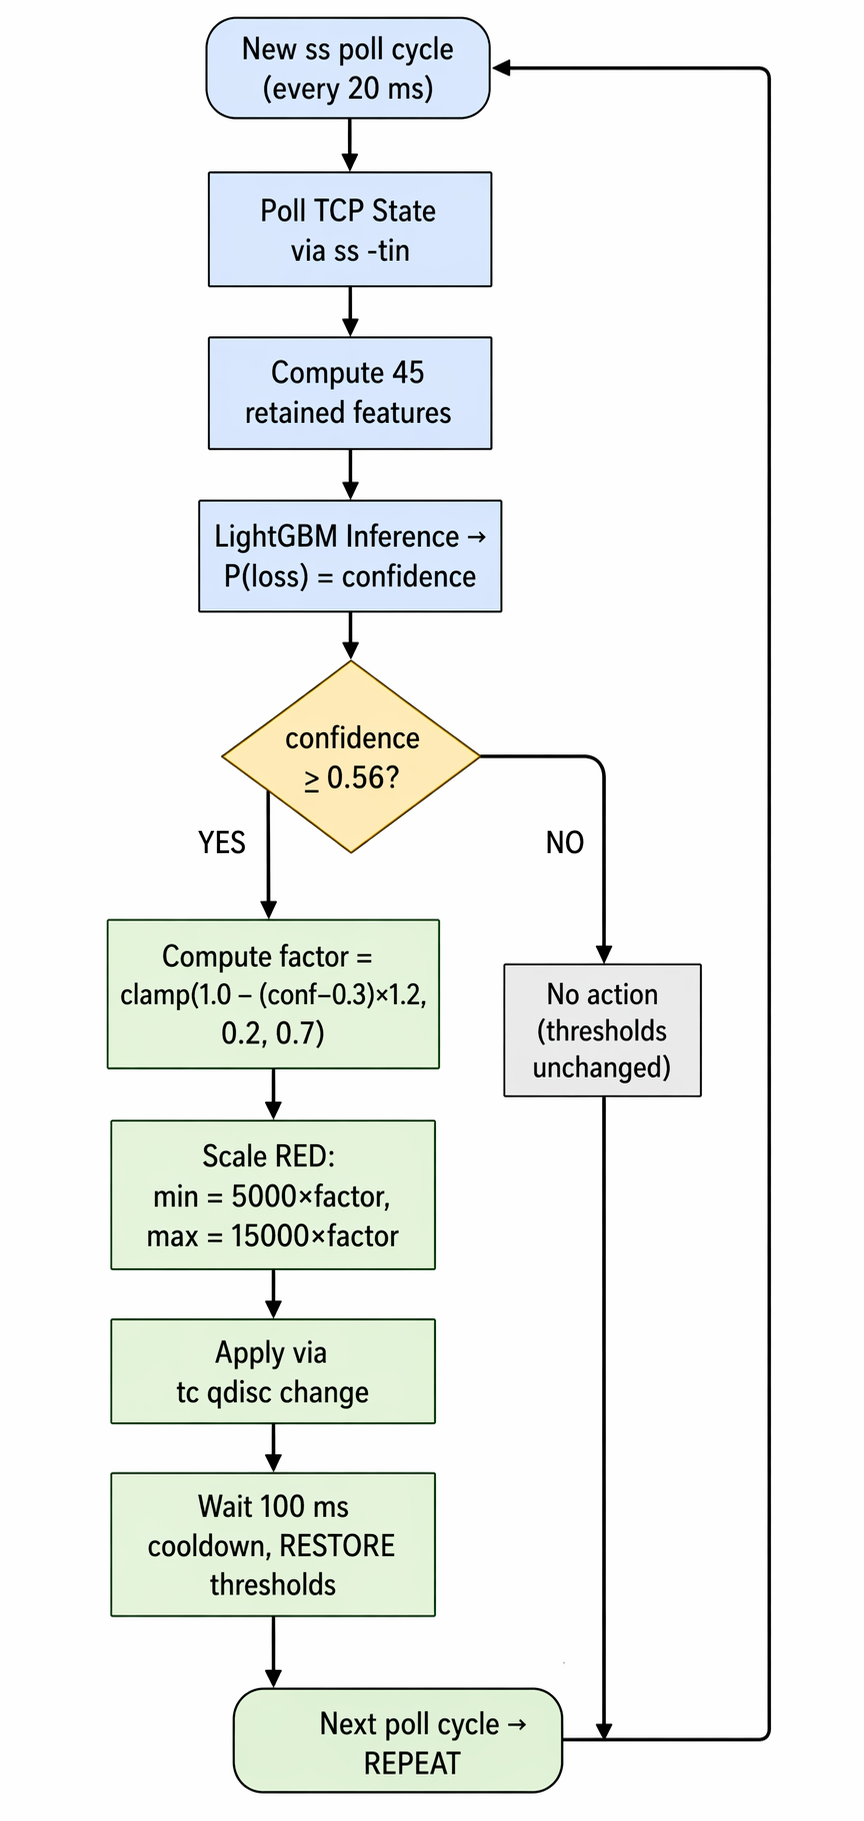
\includegraphics[width=\columnwidth]{flowchart.png}
\caption{ML-ECN Real-Time Control Loop. The daemon polls TCP state every 20\,ms, computes 45 retained features, and invokes LightGBM inference. When prediction confidence exceeds 0.56, RED thresholds are proportionally reduced; after a 100\,ms cooldown, original thresholds are restored.}
\label{fig:flowchart}
\end{figure}
